\documentclass[11pt]{article}
\usepackage[a4paper,margin=2.6cm]{geometry}
\usepackage{amsmath,amssymb,amsthm}
\usepackage{graphicx}
\graphicspath{{figures/}}
\usepackage{booktabs}
\usepackage[numbers,sort&compress]{natbib}

\usepackage[expansion=false]{microtype}
\usepackage{xcolor}
\usepackage{hyperref}
\hypersetup{colorlinks=true,linkcolor=blue!50!black,citecolor=blue!50!black,urlcolor=blue!50!black}

\newtheorem{proposition}{Proposition}
\newtheorem{corollary}{Corollary}
\theoremstyle{definition}
\newtheorem{definition}{Definition}
\theoremstyle{remark}
\newtheorem*{remark}{Remark}

\newcommand{\de}{\mathrm{de}}
\newcommand{\reff}{\rho^{\mathrm{eff}}}

\title{\textbf{Engineering Markov Blankets:\\ When Sensory States Descend from Active States}}
\author{Luca M. Possati\\ {\small University of Twente}\\ {\small\texttt{l.m.possati@utwente.nl}}}
\date{Draft v9}

\begin{document}
\maketitle

\begin{abstract}
\noindent Markov blankets are usually analysed as if the observation channel were
exogenous. In that setting, comparing boundary designs reduces to Blackwell's
comparison of experiments. A Markov blanket, however, contains active states,
and these can causally influence later sensory states. This paper studies what
changes when they do, and turns the answer into a design problem.

In a minimal multi-agent system, one observer echoes the decision agent's
previous announcement with probability $\kappa$. We compare this closed loop
with an open-loop system built to be \emph{the same experiment at every step}.
We prove four results.
(i) No criterion defined on per-step channels distinguishes the two systems.
(ii) A factorised generative model is exact in one and misspecified in the
other.
(iii) The closed loop is a sequential garbling of its step-equivalent open loop,
so even a perfectly specified agent loses decision value.
(iv) An agent that ignores the loop turns its wrong beliefs into attractors above
an analytic threshold $\kappa^\ast$.
At $\rho=0.6$, $\kappa=0.5$, $T=30$, final accuracy is 98.5\% in the open loop,
90.2\% in the closed loop for a correctly specified agent, and 76.2\% for an
agent that ignores the loop. The last ends almost certain of the wrong state in
19.3\% of episodes.

We then treat the blanket's topology as the design variable. A cost-based design
map shows when an engineer should leave the loop, cut it, or have the agent learn
it. Finally, we let the agent engineer its own blanket: before each episode it
may withhold its announcements, cutting the loop at a cost. Cutting the loop
also removes all evidence about the loop, so a greedy agent can seal its
boundary on the basis of beliefs it can never revise. We prove this lock-in is
absorbing. An agent that adds the expected information gain about its own
blanket topology to its policy value (an expected-free-energy term) avoids it.
At an intermediate cost, this agent reduces cumulative regret by 61\% (0.297 to
0.115) and adopts the oracle boundary policy in 89\% of worlds.

Engineering a Markov blanket is thus a well-posed problem. It is about locating
active-to-sensory paths, choosing whether to cut, model or learn them, and, for
an agent engineering its own boundary, preserving the ability to learn what its
boundary is.
\end{abstract}

% =====================================================================
\section{Introduction}

A Markov blanket separates internal states $\mu$ from external states $\eta$
through sensory states $s$ and active states $a$, so that
$\mu\perp\eta\mid(s,a)$
\citep{kirchhoff2018markov,dacosta2021bayesian,friston2023simpler}. The construct
is central to the Free Energy Principle (FEP) and to Active Inference
\citep{parr2022active}. Its explanatory status is also contested
\citep{biehl2021technical,bruineberg2022emperor}. A recurring worry is that a
blanket partition is merely descriptive: it can be read off a system without
doing any work in explaining that system's behaviour.

One natural way to make blankets do work is to treat them as design objects,
that is, to ask how behaviour changes when the boundary is engineered
differently. As long as the sensory channel is exogenous, however, this reduces
to a familiar problem. Comparing two sensory boundaries is then comparing two
statistical experiments, which Blackwell's theorem \citep{blackwell1953}, Lindley
information \citep{lindley1956} and Bayesian experimental design
\citep{chaloner1995} already handle. Talk of ``blankets'' adds vocabulary but no
content.

This paper identifies a case where the blanket framing does add content. What
distinguishes a Markov blanket from an observation channel is that it contains
\emph{active} states, and active states can be causal ancestors of later sensory
states. When this happens, the experiment the agent faces is no longer fixed. It
depends on what the agent has done, and hence on what the agent has believed. We
show that this property is invisible to every criterion defined on per-step
channel statistics, yet it changes both the value of the evidence stream and the
calibration of any agent that fails to represent it.

\paragraph{Contributions.} The paper makes five contributions.
\begin{enumerate}
\item \emph{Step-wise equivalence with topological difference}
      (Proposition~\ref{prop:equiv}). We construct a closed-loop boundary and an
      open-loop boundary that are identical as experiments at every step but
      differ in whether a sensory state descends from an active state.
\item \emph{Misspecification without detectable marginal error}
      (Proposition~\ref{prop:joint}). A factorised generative model is exactly
      correct for the open loop and wrong for the closed loop, although it
      matches every per-step marginal of both.
\item \emph{Sequential garbling} (Proposition~\ref{prop:garbling}). The closed
      loop is a garbling of its step-equivalent open loop, so the loop reduces
      decision value even for a perfectly specified agent.
\item \emph{Self-reinforcement threshold} (Proposition~\ref{prop:drift}). An
      agent that ignores the loop turns it into a positive-feedback system above
      an analytic threshold $\kappa^\ast$. A correctly specified agent is immune.
\item \emph{Remedies}. We compare structural, inferential and epistemic
      interventions, including an honest negative result for one-step
      expected-free-energy probing.
\item \emph{A design map} (Section~\ref{sec:engineering}). With explicit costs,
      we determine when an external designer should leave, cut or learn the
      loop.
\item \emph{Self-engineering} (Proposition~\ref{prop:sealing} and
      Section~\ref{sec:self}). An agent that can cut its own loop faces an
      epistemic trap: cutting destroys the evidence that would justify cutting.
      We prove that greedy boundary choice can seal itself permanently. We then
      show that the epistemic term of expected free energy, applied to the
      agent's uncertainty about its own blanket topology, avoids the trap.
\end{enumerate}

% =====================================================================
\section{Background and positioning}\label{sec:background}

\paragraph{Exogenous experiments.} Blackwell \citep{blackwell1953} orders
experiments by garbling: $E'$ is less informative than $E$ if $E'$ can be
generated from $E$'s output plus independent noise. Equivalently, $E$ is weakly
better in every Bayesian decision problem. Lindley's measure
\citep{lindley1956} and Bayesian experimental design \citep{chaloner1995}
quantify and optimise expected information gain. All of these results take the
experiment to be fixed before the decision maker acts.

\paragraph{Endogenous and correlated evidence.} Several literatures study
evidence that is correlated with the recipient's own past behaviour or beliefs.
\begin{itemize}
\item Herding and informational cascades
      \citep{banerjee1992,bikhchandani1992}: agents infer from others' actions,
      which themselves reflect earlier inferences.
\item Persuasion bias \citep{demarzo2003} and correlation neglect
      \citep{enke2019}: repeated or correlated signals are treated as
      independent.
\item Misspecified Bayesian learning \citep{berk1966}, and in particular
      Berk--Nash equilibrium \citep{esponda2016}: agents with wrong models whose
      actions shape the data they learn from settle on self-confirming beliefs.
\item Sensor fusion: the ``data incest'' problem of double-counting shared
      information \citep{julier1997}.
\item Neuroscience: the reafference principle and corollary discharge
      \citep{vonholst1950}, which address how organisms distinguish
      self-generated from externally generated sensation.
\end{itemize}

\paragraph{What is new here.} None of these phenomena is new, and we do not
claim otherwise. Our contribution is to locate them in a single structural
property of a Markov blanket: whether some sensory state has an active state
among its causal ancestors. We make that property precise, and we show formally
that it escapes per-step channel comparison. We then treat the property as an
engineering variable that admits three kinds of remedy: changing the topology,
changing the model, or learning the topology.

% =====================================================================
\section{Model}\label{sec:model}

\subsection{Agents and states}

A binary external state $\eta\in\{0,1\}$ is drawn uniformly and fixed within an
episode of $T$ steps. At each step $t$ the decision agent receives
$s_t=(s_{1,t},s_{2,t})$, updates its belief $q_t(\eta)$, and emits an
announcement
\begin{equation}
a_t=\arg\max_\eta q_t(\eta),
\end{equation}
with ties broken uniformly. The announcement is an active state: it is part of
the agent's blanket and is observable by others. Observer $A_1$ always reports
an independent observation of reliability $\rho\in(1/2,1)$, so that
$P(s_{1,t}=\eta\mid\eta)=\rho$.

\subsection{Two boundary organisations}

\begin{definition}[Closed loop, system A]
Observer $A_2$ can see the decision agent's announcements. At each $t\ge2$,
independently with probability $\kappa\in[0,1)$, it repeats the previous
announcement; otherwise it reports its own independent observation $z_{2,t}$
of reliability $\rho$:
\begin{equation}
s_{2,t}=C_t\,a_{t-1}+(1-C_t)\,z_{2,t},\qquad C_t\sim\mathrm{Bern}(\kappa).
\label{eq:loop}
\end{equation}
At $t=1$ there is no previous announcement, and $s_{2,1}=z_{2,1}$.
\end{definition}

Let $\alpha_{t}=P(a_{t}=\eta\mid\eta)$ denote the accuracy of the announcement
process. By the symmetry of the model, $\alpha_t$ does not depend on the value of
$\eta$.

\begin{definition}[Step-matched open loop, system B]
Observer $A_2$ is an independent sensor whose reliability at step $t$ is
\begin{equation}
\reff_t=\kappa\,\alpha_{t-1}+(1-\kappa)\,\rho\quad(t\ge2),\qquad \reff_1=\rho.
\label{eq:reff}
\end{equation}
\end{definition}

System B is defined relative to the announcement process of A. It is the open
loop that reproduces A's per-step statistics exactly.

\paragraph{Blanket topology.} In A, $s_{2,t}\in\de(a_{t-1})$: a sensory state
descends from an active state. The path
$s_{<t}\to\mu_{t-1}\to a_{t-1}\to s_{2,t}$ connects past and present sensory
states without passing through $\eta$. In B no such path exists. The two systems
share the same state partition. What differs is the causal topology of the
blanket: whether the arrows run from active to sensory states.

\subsection{Agents}

\begin{definition}[Naive agent]
The naive agent uses the factorised likelihood
\begin{equation}
p_{\text{naive}}(s_{1:t}\mid\eta)=\prod_{\tau\le t}p(s_{1,\tau}\mid\eta)\,
\mathrm{Bern}_{\reff_\tau}(s_{2,\tau}\mid\eta),
\end{equation}
with the exact per-step marginal reliability $\reff_\tau$. In A we compute
$\reff$ as a self-consistent fixed point: the reliability the naive agent's own
announcements induce. The naive agent is therefore correct about every per-step
marginal it could check, and its model is the best-fitting independent model of
the data it generates, in the spirit of \citep{esponda2016}.
\end{definition}

\begin{definition}[Aligned agent]
The aligned agent represents the active-to-sensory path, as an efference copy
would:
\begin{equation}
p(s_{2,t}\mid\eta,a_{t-1})=\kappa\,\mathbb{1}[s_{2,t}=a_{t-1}]+(1-\kappa)\,
\rho^{\mathbb{1}[s_{2,t}=\eta]}(1-\rho)^{\mathbb{1}[s_{2,t}\neq\eta]}.
\label{eq:aligned}
\end{equation}
\end{definition}

% =====================================================================
\section{Theory}\label{sec:theory}

\begin{proposition}[Step-wise experimental equivalence]\label{prop:equiv}
For every $t$, $p_A(s_t\mid\eta)=p_B(s_t\mid\eta)$. Consequently, no criterion
defined on the family of per-step channels $\{p(s_t\mid\eta)\}_{t\le T}$
distinguishes A from B. This includes the Blackwell ordering of per-step
experiments, per-step Lindley information and one-step value of information.
\end{proposition}

\begin{proof}
The announcement $a_{t-1}$ is a function of $s_{1:t-1}$ and of tie-breaking
noise. Given $\eta$, these are independent of the current draws $s_{1,t}$,
$z_{2,t}$ and $C_t$. Hence $s_{1,t}\perp s_{2,t}\mid\eta$ in A, as in B. By
\eqref{eq:loop},
$P_A(s_{2,t}=\eta\mid\eta)=\kappa\alpha_{t-1}+(1-\kappa)\rho=\reff_t$, which by
\eqref{eq:reff} equals $P_B(s_{2,t}=\eta\mid\eta)$. The component $s_{1,t}$ has
the same law in both systems.
\end{proof}

\begin{proposition}[Joint non-equivalence and misspecification]\label{prop:joint}
Let $\kappa>0$ and $0<\alpha_{t-1}<1$. Then
$\mathrm{Cov}_A(s_{2,t},a_{t-1}\mid\eta)=\kappa\,\mathrm{Var}(a_{t-1}\mid\eta)>0$,
whereas $\mathrm{Cov}_B(s_{2,t},a_{t-1}\mid\eta)=0$. Hence
$p_A(s_{1:T}\mid\eta)\neq p_B(s_{1:T}\mid\eta)$ for $T\ge2$. The factorised
likelihood of the naive agent is exactly correct in B and misspecified in A.
\end{proposition}

\begin{proof}
Given $\eta$, both $C_t$ and $z_{2,t}$ are independent of $a_{t-1}$. Therefore
$\mathrm{Cov}(C_ta_{t-1}+(1-C_t)z_{2,t},\,a_{t-1}\mid\eta)=
\kappa\,\mathrm{Var}(a_{t-1}\mid\eta)$, which is positive when
$0<\alpha_{t-1}<1$. In B, $s_{2,t}$ is independent of the past given $\eta$.
\end{proof}

Propositions~\ref{prop:equiv} and~\ref{prop:joint} together say that the
difference between A and B is invisible step by step but real over histories.
The next result says that it matters even to an agent who models it correctly.

\begin{proposition}[The closed loop is a sequential garbling]\label{prop:garbling}
Suppose $\alpha_{t-1}\ge\rho$ for all $t\ge2$. Then the history experiment
$s_{1:T}$ of system A is a garbling of the history experiment of system B, where
B is matched to A's announcement process. Hence, for every decision problem
based on the history and every prior, the Bayes-optimal expected utility under A
is at most that under B.
\end{proposition}

\begin{proof}
We generate A's history from B's history and independent noise, step by step.
The $s_1$ components are copied. Given B's output $s^B_{2,t}$, which has
reliability $\reff_t\ge\rho$ because $\alpha_{t-1}\ge\rho$, flip it with
probability
\begin{equation}
\phi_t=\frac{\reff_t-\rho}{2\reff_t-1}\in[0,\tfrac12).
\end{equation}
This yields an independent reliability-$\rho$ observation $\tilde z_{2,t}$. Then,
with independent probability $\kappa$, replace it by $a_{t-1}$. Here $a_{t-1}$
is computed by running A's announcement rule on the already constructed history
$\tilde s_{1:t-1}$, which is a function of B's outputs and earlier noise. By
induction on $t$, the constructed sequence has exactly the law of A's history.
Blackwell's theorem \citep{blackwell1953} gives the value inequality.
\end{proof}

\begin{remark}
Proposition~\ref{prop:garbling} turns the step-wise equivalence of
Proposition~\ref{prop:equiv} into a sequential inequality. The loop spends
channel capacity re-transmitting the agent's own past output. This part of the
signal carries no information about $\eta$ beyond what the agent already has.
The condition $\alpha_{t-1}\ge\rho$ holds in all our runs.
\end{remark}

\begin{proposition}[Self-reinforcement threshold]\label{prop:drift}
Consider the naive agent in A with log-odds $\ell_t$ in favour of its current
announcement. Suppose that announcement is wrong, $a_{t-1}\neq\eta$, and let
$r=\reff_t$. The expected one-step change of $\ell$ in favour of the wrong state
is
\begin{equation}
\Delta_{\text{naive}}=\kappa\,\mathrm{logit}(r)-(2\rho-1)\big[\mathrm{logit}(\rho)
+(1-\kappa)\,\mathrm{logit}(r)\big],
\label{eq:drift}
\end{equation}
which is positive if and only if
\begin{equation}
\kappa>\kappa^\ast(\rho,r)=\frac{(2\rho-1)\big[\mathrm{logit}(\rho)+\mathrm{logit}(r)\big]}
{2\rho\,\mathrm{logit}(r)}.
\label{eq:kstar}
\end{equation}
For the aligned agent, the expected one-step change of its log-odds in favour of
the true state equals a Kullback--Leibler divergence between its likelihoods
under $\eta$ and $\neg\eta$. This is strictly positive because $s_1$ is always
informative. Its wrong beliefs are therefore never self-reinforcing in
expectation.
\end{proposition}

\begin{proof}
The component $s_{1,t}$ contributes $-(2\rho-1)\,\mathrm{logit}(\rho)$ in
expectation. With probability $\kappa$, $s_{2,t}=a_{t-1}$, which the naive agent
scores as $+\mathrm{logit}(r)$. With probability $1-\kappa$, $s_{2,t}$ is an
independent reliability-$\rho$ report, which contributes
$-(2\rho-1)\,\mathrm{logit}(r)$ in expectation. Summing gives \eqref{eq:drift},
and solving $\Delta_{\text{naive}}=0$ for $\kappa$ gives \eqref{eq:kstar}. For
the aligned agent, the expected log-likelihood ratio under the true model is a
KL divergence. It is non-negative, and strictly positive because the $s_1$ term
alone contributes $\mathrm{KL}(\mathrm{Bern}_\rho\|\mathrm{Bern}_{1-\rho})>0$.
\end{proof}

When the announcement is correct, the loop pushes the naive agent toward the
truth as well. Above $\kappa^\ast$, both correct and incorrect beliefs are
therefore self-reinforcing: the naive agent becomes a bistable system that locks
in on whichever state it favours early.

% =====================================================================
\section{Simulation results}\label{sec:results}

\paragraph{Design.} Unless stated otherwise: $\rho=0.60$, $\kappa=0.50$, $T=30$,
$N=200{,}000$ episodes, seed 20260930. We use common random numbers across
conditions. $\reff$ is computed as the naive agent's self-consistent fixed point
in A. It rises from 0.600 to 0.681 over the episode.

For system A we report the naive and the aligned agent. Each generates its own
announcements and hence its own loop. For system B we report the naive agent,
which is exactly specified there. The comparator B is matched to the naive
agent's announcement process. In all runs the aligned agent's announcement
accuracy is at least that of the naive agent, so a comparator matched to the
aligned agent would be at least as informative as B. The A-aligned versus B gap
reported below is therefore conservative.

\subsection{Equivalence, value loss and miscalibration}

The largest per-step difference between the empirical marginals
$P(s_{2,t}=\eta)$ in A and B is $0.0021$. This is Monte Carlo noise, as
Proposition~\ref{prop:equiv} requires.

\begin{table}[h]
\centering
\begin{tabular}{lcccc}
\toprule
Condition & Accuracy & Mean confidence & Lock-in & Log-loss \\
\midrule
B, open loop, naive (exact)   & 0.985 & 0.985 & 0.0006 & 0.041\\
A, closed loop, aligned       & 0.902 & 0.902 & 0.0010 & 0.237\\
A, closed loop, naive         & 0.762 & 0.995 & 0.193  & 1.838\\
\bottomrule
\end{tabular}
\caption{Final step ($T=30$). Lock-in is the fraction of episodes ending with
$q(\eta_{\text{true}})<0.01$. A and B are identical experiments at every step.}
\label{tab:main}
\end{table}

\begin{figure}[t]
\centering
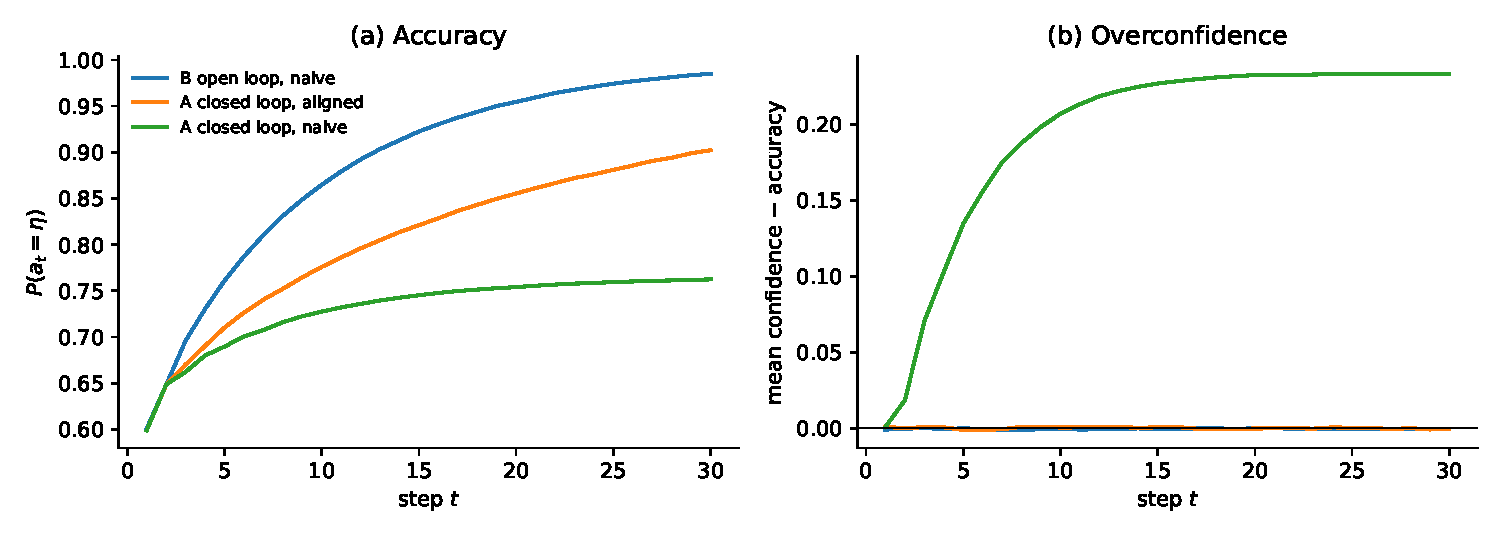
\includegraphics[width=\linewidth]{fig1_equivalence.pdf}
\caption{Step-wise equivalent boundaries with different topology. (a) Accuracy
over time. (b) Mean confidence minus accuracy. Only the naive agent in the closed
loop is miscalibrated.}
\label{fig:equiv}
\end{figure}

Table~\ref{tab:main} and Figure~\ref{fig:equiv} give three results.

\emph{Result 1: topology reduces value, even with a correct model.} The aligned
agent in A reaches 90.2\% accuracy against 98.5\% in B, with identical per-step
channels. This is Proposition~\ref{prop:garbling} made quantitative.

\emph{Result 2: ignoring the topology produces confident error.} The naive agent
in A reports a mean confidence of 0.995 while being right only 76.2\% of the
time. It ends with more than 99\% confidence in the wrong state in 19.3\% of
episodes. The same model is perfectly calibrated in B.

\emph{Result 3: early errors become permanent.} In A the naive agent is wrong at
step 10 in 27.3\% of episodes. Of those, 85.6\% are still wrong at step 30. For
the aligned agent the corresponding persistence is 26.7\%. In B it is 6.5\%.

\subsection{Dependence on $\kappa$ and robustness}

\begin{figure}[t]
\centering
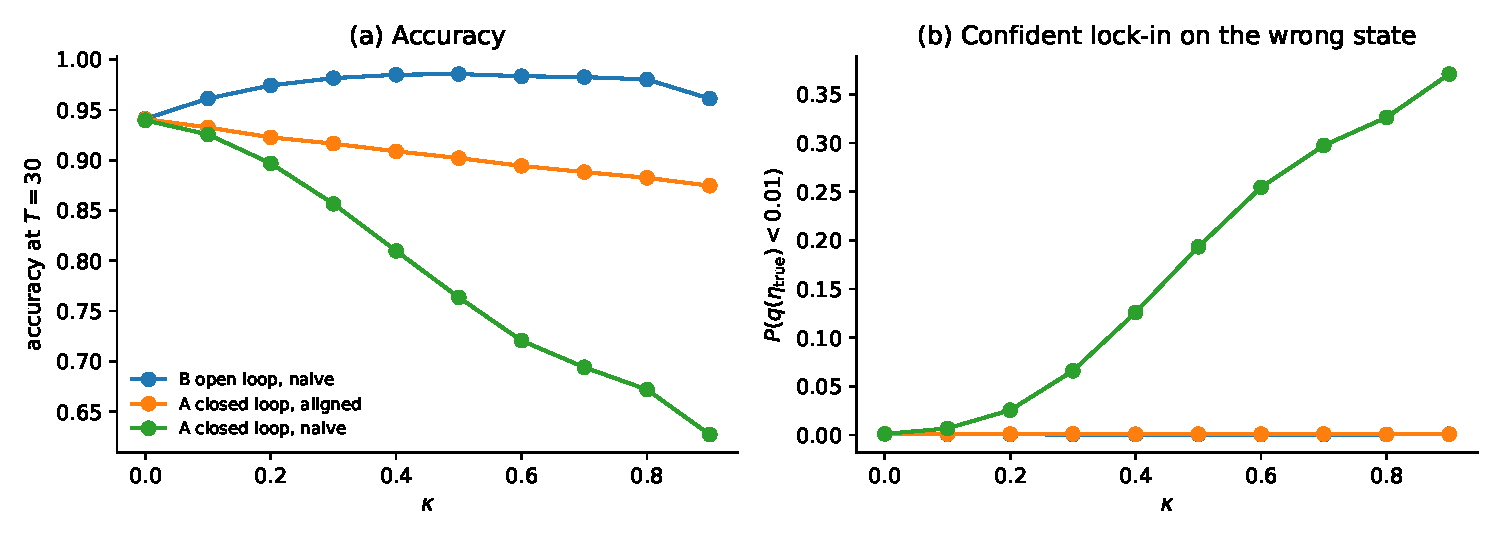
\includegraphics[width=\linewidth]{fig2_kappa_sweep.pdf}
\caption{Sweep over the loop strength $\kappa$ ($N=100{,}000$ per point). At
$\kappa=0$ all conditions coincide.}
\label{fig:sweep}
\end{figure}

At $\kappa=0$ all conditions coincide (accuracy 0.940--0.941), as they must;
Figure~\ref{fig:sweep} shows the full sweep. As $\kappa$ increases from 0.1 to
0.9:
\begin{itemize}
\item naive accuracy in A falls from 0.926 to 0.627, and lock-in rises from
      0.007 to 0.371;
\item the aligned agent degrades gradually, from 0.932 to 0.875, with lock-in
      never above 0.0013;
\item the matched open loop B stays between 0.961 and 0.986.
\end{itemize}
The same pattern holds across sensory reliability at $\kappa=0.5$
(Table~\ref{tab:rho}).

\begin{table}[h]
\centering
\begin{tabular}{lccc}
\toprule
& $\rho=0.55$ & $\rho=0.60$ & $\rho=0.70$\\
\midrule
B, naive (exact)      & 0.859 & 0.986 & 1.000\\
A, aligned            & 0.737 & 0.902 & 0.996\\
A, naive              & 0.637 & 0.764 & 0.936\\
A, naive: lock-in     & 0.175 & 0.193 & 0.054\\
\bottomrule
\end{tabular}
\caption{Final accuracy at $\kappa=0.5$ for three sensory reliabilities
($N=100{,}000$).}
\label{tab:rho}
\end{table}

\subsection{The self-reinforcement threshold}

\begin{figure}[t]
\centering
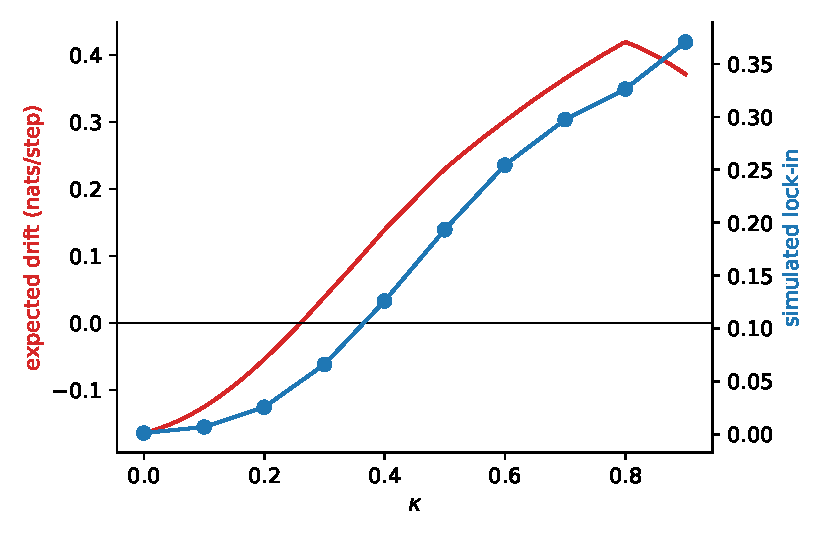
\includegraphics[width=0.62\linewidth]{fig3_threshold.pdf}
\caption{Analytic expected drift toward the wrong state for the naive agent
(Eq.~\ref{eq:drift}, left axis) and simulated lock-in (right axis).}
\label{fig:thr}
\end{figure}

We evaluate Eq.~\eqref{eq:kstar} at the late-episode value of $\reff$ for each
$\kappa$. This gives $\kappa^\ast\in[0.25,0.30]$. The analytic drift changes
sign between $\kappa=0.2$ ($\Delta=-0.054$ nats per step) and $\kappa=0.3$
($\Delta=+0.039$) (Figure~\ref{fig:thr}). Simulated lock-in accelerates in
exactly this interval: 0.026, then 0.066, then 0.126 at $\kappa=0.2,0.3,0.4$.
Below the threshold, lock-in is small but non-zero, because of finite-horizon
fluctuations. The threshold marks where confident error stops being a transient
and becomes an attractor.

% =====================================================================
\section{Three remedies}\label{sec:remedies}

The same defect admits interventions of three different kinds.
\begin{description}
\item[Structural.] Change the blanket topology by cutting $a\to z_2$, so that
      $\kappa=0$.
\item[Inferential.] Keep the topology and align the generative model, using
      Eq.~\eqref{eq:aligned} with the known $\kappa$.
\item[Epistemic.] Keep the topology and let the agent learn it. The agent holds
      a joint belief over $(\eta,\kappa)$ on the grid
      $\kappa\in\{0,0.1,\dots,0.9\}$, with a uniform prior.
\end{description}

We test three variants of the epistemic learner.
\begin{itemize}
\item \emph{Passive}: always announce the most probable state.
\item \emph{Random probes}: announce a uniformly random state with probability
      $\varepsilon$.
\item \emph{EFE probes}: choose the announcement $x$ by minimising a one-step
      reduced expected free energy
      \begin{equation}
      G(x)=\underbrace{1-q(\eta=x)}_{\text{risk}}
      -\beta\,\underbrace{\mathbb{E}_{q(o\mid x)}\big[D_{\mathrm{KL}}(q(\eta,\kappa\mid o,x)\,\|\,q(\eta,\kappa))\big]}_{\text{information gain on states and parameters}}.
      \end{equation}
      This contains the parameter-information (``novelty'') term of Active
      Inference \citep{friston2017curiosity,schwartenbeck2019}.
\end{itemize}
Announcing against one's current belief is informative about $\kappa$: an echo
of a contrarian announcement is distinguishable from independent evidence.
Probing therefore trades announcement accuracy for structural information.

\begin{table}[h]
\centering
\begin{tabular}{lcccc}
\toprule
Remedy & Final acc. & Ann.\ acc. & Probe rate & $|\hat\kappa-\kappa|$\\
\midrule
None (naive)                          & 0.762 & -- & -- & --\\
Structural (cut loop)                 & 0.940 & -- & -- & --\\
Inferential (known $\kappa$)          & 0.902 & -- & -- & --\\
Epistemic, passive                    & 0.890 & 0.798 & 0 & 0.127\\
Epistemic, random $\varepsilon=0.1$   & 0.891 & 0.771 & 0.050 & 0.126\\
Epistemic, random $\varepsilon=0.3$   & 0.897 & 0.712 & 0.150 & 0.123\\
Epistemic, EFE $\beta=1$              & 0.892 & 0.799 & 0.007 & 0.127\\
Epistemic, EFE $\beta=4$              & 0.891 & 0.800 & 0.013 & 0.127\\
\bottomrule
\end{tabular}
\caption{Remedies at $\rho=0.6$, $\kappa=0.5$, $T=30$ ($N=50{,}000$). ``Ann.\
acc.'' is the mean per-step accuracy of announcements, which is the pragmatic
cost of probing.}
\label{tab:remedies}
\end{table}

\begin{figure}[t]
\centering
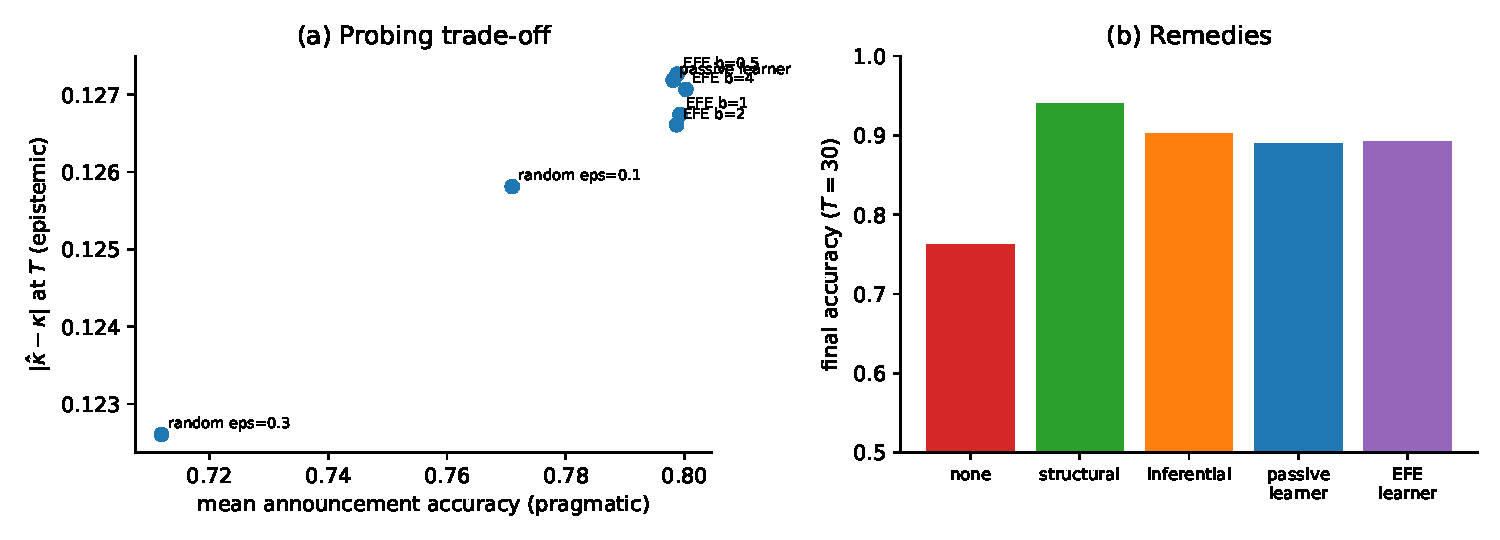
\includegraphics[width=\linewidth]{fig4_remedies.pdf}
\caption{(a) Pragmatic cost versus structural information for probing
strategies. (b) Final accuracy under the three remedies.}
\label{fig:rem}
\end{figure}

Table~\ref{tab:remedies} and Figure~\ref{fig:rem} give three results.

\emph{Result 4: the structural remedy dominates in accuracy.} Cutting the loop
(94.0\%) beats modelling it (90.2\%). This follows from
Proposition~\ref{prop:garbling}: modelling the loop lets the agent discount
echoes, but only cutting it restores the fresh evidence those echoes displaced.
Whether cutting is optimal therefore depends on its cost relative to modelling.
This is the engineering trade-off.

\emph{Result 5: learning the topology passively recovers most of the loss.}
Holding uncertainty over $\kappa$ and marginalising, without any probing,
already gives 89.0\%. That is 91\% of the gap between the naive agent (76.2\%)
and the agent that knows $\kappa$ (90.2\%). The same holds at $\kappa=0.2$
(0.920 against 0.923 known and 0.898 naive) and at $\kappa=0.8$ (0.875 against
0.883 known and 0.673 naive). The crucial step is representing the possibility
of a loop, not knowing its strength.

\emph{Result 6: one-step EFE probing is almost never worth it here.} The EFE
agent probes in under 1.5\% of steps even at $\beta=4$, and its accuracy is
indistinguishable from the passive learner's. Random probing at
$\varepsilon=0.3$ improves final accuracy by 0.7 points, but it costs 8.6 points
of announcement accuracy, and the posterior over $\kappa$ remains broad (entropy
$\approx1.83$ nats against a maximum of $\ln10\approx2.30$). By its own
criterion, the EFE agent is right not to probe. With one-step lookahead, the
information about $\kappa$ gained from a single contrarian announcement is small
compared with its immediate risk.

We read Result 6 as a genuine negative result about myopic epistemic action, not
as a failure of the framework. The benefit of knowing $\kappa$ accrues over many
future steps, and a one-step objective cannot see it. Multi-step policies, or
longer interactions in which $\kappa$ persists across episodes, are the natural
setting in which active probing of one's own blanket should pay off. We leave
this to future work.

% =====================================================================
\section{Engineering the blanket}\label{sec:engineering}

The previous section compared remedies by accuracy alone. Engineering requires
costs. We now treat the blanket's topology as the design variable, first from
the perspective of an external designer, and then from the perspective of the
agent itself.

\subsection{A design map}

An external designer chooses one of three configurations for a system with loop
strength $\kappa$:
\begin{itemize}
\item \emph{none}: leave the loop and a naive agent, at no cost;
\item \emph{cut}: remove the path $a\to z_2$, at cost $C_{\text{cut}}$;
\item \emph{learn}: keep the loop and equip the agent with the joint
      $(\eta,\kappa)$ model, at cost $C_{\text{model}}$ (computation, memory,
      model complexity).
\end{itemize}
The design objective is
\begin{equation}
J(d;\kappa)=\big[1-\mathrm{Acc}_d(\kappa)\big]+C_d,
\qquad d^\ast(\kappa)=\arg\min_d J(d;\kappa),
\label{eq:design}
\end{equation}
where the accuracies are the simulated final accuracies at $T=30$.

\begin{figure}[t]
\centering
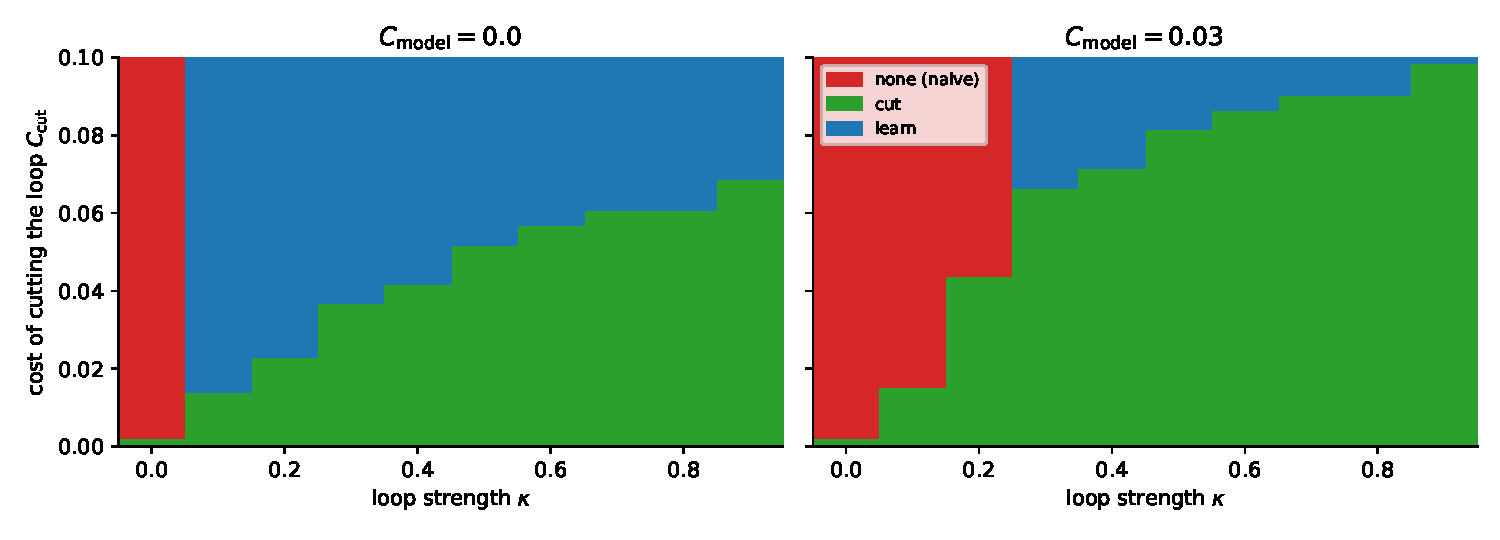
\includegraphics[width=\linewidth]{fig5_design_map.pdf}
\caption{Design map. The optimal blanket configuration as a function of loop
strength $\kappa$ and the cost of cutting the loop, for two costs of the richer
generative model.}
\label{fig:map}
\end{figure}

Figure~\ref{fig:map} shows three regimes.
\begin{itemize}
\item When $\kappa\approx0$, doing nothing is optimal: there is no loop to
      remedy.
\item When cutting is cheap relative to the damage the loop causes, cutting
      wins. Its region grows with $\kappa$, because the value lost to the loop
      grows with $\kappa$ (Proposition~\ref{prop:garbling}).
\item When cutting is expensive, learning wins, unless the model cost exceeds
      what the loop destroys. With $C_{\text{model}}=0.03$, leaving a weak loop
      ($\kappa\le0.2$) unmodelled becomes optimal.
\end{itemize}
This is the analogue, for blanket topology, of the communication-cost
trade-off in classical sensor design. Here, though, the benefit side is
governed by the sequential results of Section~\ref{sec:theory}, not by per-step
channel comparison.

\subsection{Self-engineering: the agent chooses its own boundary}\label{sec:self}

We now remove the external designer. The agent lives through a sequence of
$M=40$ episodes in a world whose loop strength $\kappa$ is fixed but unknown.
$\eta$ is redrawn in each episode. Before each episode the agent chooses a
boundary configuration:
\begin{itemize}
\item \emph{visible}: its announcements are observable, so the loop, of unknown
      strength, is active;
\item \emph{hidden}: it withholds its announcements, which cuts the loop, at a
      cost $C$ per episode.
\end{itemize}
Within an episode the agent is the joint $(\eta,\kappa)$ learner of
Section~\ref{sec:remedies}. Its belief $q(\kappa)$ is carried across episodes.

\paragraph{Policy selection.} The agent evaluates the two boundary policies with
\begin{align}
G(\text{visible}) &= \mathbb{E}_{q(\kappa)}\big[1-\mathrm{Acc}_{\text{learn}}(\kappa)\big]
  -\beta\,\mathcal{I}_\kappa(\text{visible}),\label{eq:Gvis}\\
G(\text{hidden}) &= \big[1-\mathrm{Acc}_{\text{hidden}}\big]+C,\label{eq:Ghid}
\end{align}
and chooses the minimum. Here $\mathcal{I}_\kappa(\text{visible})$ is the
expected information gain about $\kappa$ from one visible episode. It is
estimated by Monte Carlo from a bank of simulated episodes: $\kappa$ is sampled
from $q$, a simulated episode is drawn, and $q$ is updated with that episode's
likelihood over $\kappa$. The case $\beta=0$ is greedy expected utility. For
$\beta>0$ the objective contains the epistemic, parameter-information term of
expected free energy \citep{friston2017curiosity,schwartenbeck2019}, applied to
the agent's uncertainty about the topology of its own blanket.

\begin{proposition}[Self-sealing boundaries]\label{prop:sealing}
Under the hidden configuration, the likelihood of every episode is constant in
$\kappa$, so $q(\kappa)$ is unchanged. Consequently, if a greedy agent
($\beta=0$) chooses \emph{hidden} at some episode, it chooses \emph{hidden} at
every later episode, whatever the true $\kappa$.
\end{proposition}

\begin{proof}
When announcements are withheld, $s_{2,t}$ is an independent reliability-$\rho$
report for every value of $\kappa$. The episode likelihood therefore factorises
into a term in $\eta$ and a term constant in $\kappa$, and the posterior over
$\kappa$ equals the prior. With $\beta=0$, both \eqref{eq:Gvis} and
\eqref{eq:Ghid} depend on the history only through $q(\kappa)$, which no longer
changes. The inequality that selected \emph{hidden} is therefore reproduced at
every later episode.
\end{proof}

Proposition~\ref{prop:sealing} is the engineering counterpart of
Proposition~\ref{prop:drift}. There, an agent that ignores its loop locks into a
wrong belief about the world. Here, an agent that cuts its loop too early locks
into an unrevisable belief about itself. Cutting is the best remedy for the
loop's informational damage (Result~4), but it is epistemically blind: it
removes the only evidence about whether it was needed. For $\beta>0$,
$\mathcal{I}_\kappa(\text{visible})>0$ whenever $q(\kappa)$ is not degenerate.
This lowers $G(\text{visible})$, so the agent keeps its boundary open long
enough to learn what it is.

\paragraph{Setup.} We simulate 3{,}000 worlds, with 300 for each
$\kappa\in\{0,0.1,\dots,0.9\}$. The prior over $\kappa$ is uniform, and $M=40$
episodes of $T=30$ steps are run for each world. Regret is measured against an
oracle that knows $\kappa$ and chooses the better of the known-$\kappa$ agent and
the hidden configuration. Utility per episode is final correctness minus $C$ if
hidden.

\begin{table}[h]
\centering
\begin{tabular}{lcccccc}
\toprule
& \multicolumn{2}{c}{$C=0.01$} & \multicolumn{2}{c}{$C=0.03$} & \multicolumn{2}{c}{$C=0.05$}\\
\cmidrule(lr){2-3}\cmidrule(lr){4-5}\cmidrule(lr){6-7}
Policy & Regret & Match & Regret & Match & Regret & Match\\
\midrule
Always visible         & 1.078 & 0.20 & 0.519 & 0.40 & 0.180 & 0.70\\
Always hidden          & 0.057 & 0.80 & 0.297 & 0.60 & 0.759 & 0.30\\
Greedy ($\beta=0$)     & 0.057 & 0.80 & 0.297 & 0.60 & 0.152 & 0.76\\
EFE, $\beta=0.05$      & 0.080 & 0.85 & \textbf{0.115} & 0.87 & 0.163 & 0.81\\
EFE, $\beta=0.1$       & 0.060 & 0.89 & 0.116 & 0.89 & \textbf{0.115} & 0.83\\
EFE, $\beta=0.2$       & 0.180 & 0.92 & 0.167 & 0.91 & 0.144 & 0.85\\
\bottomrule
\end{tabular}
\caption{Self-engineering over 40 episodes. Regret is cumulative, relative to
the oracle. Match is the fraction of worlds whose policy over the last five
episodes coincides with the oracle's.}
\label{tab:self}
\end{table}

\begin{figure}[t]
\centering
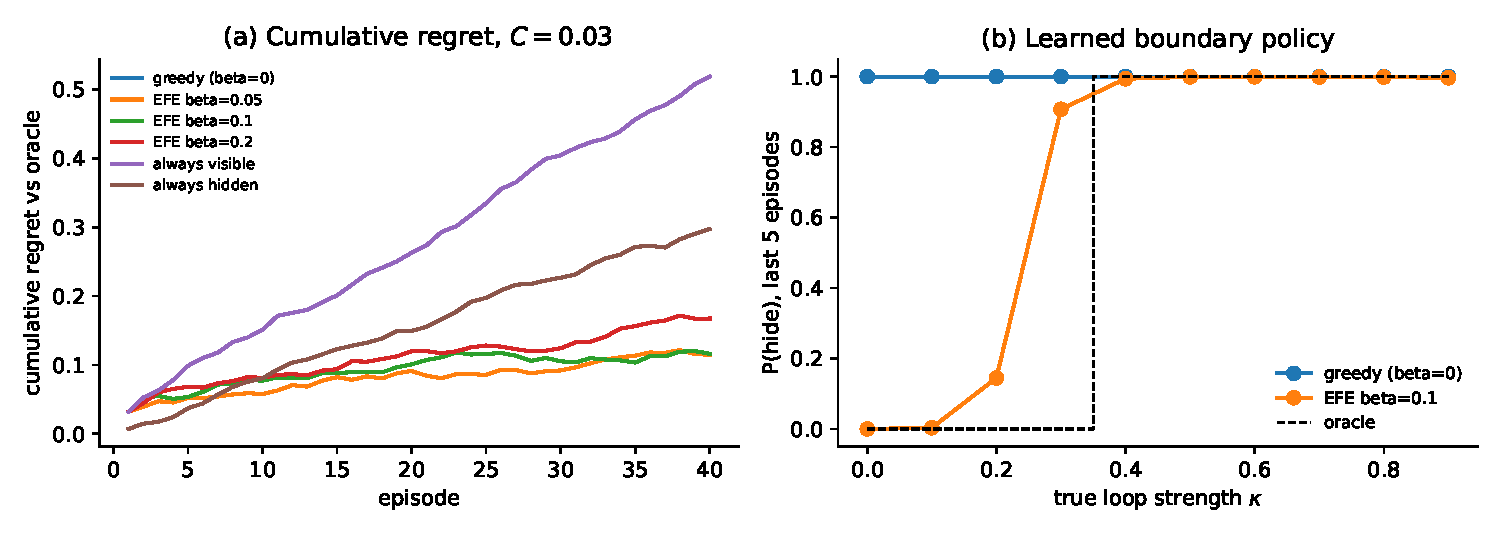
\includegraphics[width=\linewidth]{fig6_self_engineering.pdf}
\caption{Self-engineering at $C=0.03$. (a) Cumulative regret. The greedy agent
coincides with ``always hidden''. (b) Probability of hiding over the last five
episodes as a function of the true $\kappa$, against the oracle policy.}
\label{fig:self}
\end{figure}

Table~\ref{tab:self} and Figure~\ref{fig:self} give three results.

\emph{Result 7: greedy self-engineering seals itself.} At $C=0.03$, the greedy
agent's prior expected gain from hiding exceeds the cost. It therefore hides in
every world from the first episode and never stops, exactly as
Proposition~\ref{prop:sealing} predicts. Its posterior entropy over $\kappa$
stays at its maximum ($\ln10\approx2.30$). It pays for a cut it does not need
in the 40\% of worlds where $\kappa\le0.3$, and it is indistinguishable from
``always hidden'' (regret 0.297).

\emph{Result 8: the epistemic term breaks the seal.} With $\beta=0.05$ or $0.1$,
the agent starts visible in every world, learns $\kappa$, and then hides
selectively. Regret falls from 0.297 to 0.115, a 61\% reduction. The final
boundary policy matches the oracle in 89\% of worlds (Figure~\ref{fig:self}b).
Worlds with $\kappa\le0.1$ stay open, worlds with $\kappa\ge0.4$ close, and
disagreements concentrate at the boundary $\kappa\in\{0.2,0.3\}$. There, the
agent's own forecast, which is based on the passive learner's accuracy, is
slightly more pessimistic about the open loop than the oracle is. At $C=0.05$
the greedy agent happens to start visible and learns passively. Even so, the
epistemic term reduces regret by 24\% (0.152 to 0.115).

\emph{Result 9: exploration has a price.} When cutting is cheap ($C=0.01$),
hiding is optimal in 80\% of worlds, and greedy sealing is close to optimal
(regret 0.057). A moderate epistemic weight matches it ($\beta=0.1$: 0.060).
A large weight over-explores and triples regret ($\beta=0.2$: 0.180). The
epistemic term is valuable exactly when an irreversible-looking structural
choice would otherwise be made under uncertainty, and not by default.

\paragraph{Reconciling Results 6 and 8.} One-step expected-free-energy probing
within an episode was almost never worth it (Result~6). Epistemic value at the
level of boundary policies across episodes is decisive (Result~8). The
difference is the timescale at which the information is used. A single
contrarian announcement yields little information about $\kappa$ relative to
its immediate cost. A whole visible episode yields enough to decide a
configuration that will be kept for many episodes. Epistemic action about one's
own blanket pays off at the timescale at which the blanket itself is
reconfigured.

% =====================================================================
\section{Discussion}\label{sec:discussion}

\paragraph{What the blanket framing contributes.} Propositions
\ref{prop:equiv}--\ref{prop:garbling} identify a property of a boundary that
matters for inference and value but cannot be recovered from its per-step
channel statistics. That property is the presence of active states among the
causal ancestors of sensory states. It is precisely the feature that separates a
Markov blanket from an exogenous observation channel. In this setting the
blanket is not a relabelling of the channel. It is the object whose topology
determines whether per-step channel analysis is valid at all.

\paragraph{A design principle.} The results suggest a simple principle for
engineering blankets:
\begin{quote}
\emph{For every sensory state, determine whether it has active-state ancestors.
Where it does, either cut the path, model it, or learn it. If the system
chooses for itself, do not let it cut what it has not yet learned.}
\end{quote}
The three options differ in cost and effectiveness. Cutting restores
information. Modelling restores calibration but not information. Learning
restores most of the calibration without prior knowledge of the loop strength.
The design map (Figure~\ref{fig:map}) makes the choice among them a cost-benefit
calculation. The last clause of the principle is Proposition~\ref{prop:sealing}:
structural remedies are epistemically blind, so a self-engineering system must
value information about its own boundary before closing it.

\paragraph{Relation to Active Inference.} In Active Inference, beliefs about the
consequences of one's own actions are part of the generative model
\citep{parr2022active,friston2015epistemic}. Our results make one such belief
explicit: how much of what I sense is my own echo. The aligned model
\eqref{eq:aligned} is a minimal efference copy \citep{vonholst1950}. The joint
$(\eta,\kappa)$ learner is a minimal form of structure learning. The
self-engineering agent of Section~\ref{sec:self} goes one step further. It
selects policies over its own blanket topology, and the epistemic term of
expected free energy, applied to uncertainty about that topology, is what
prevents it from sealing its boundary on unrevisable beliefs. The contrast
between Results~6 and~8 locates where epistemic value about one's own blanket
matters: at the timescale at which the blanket is reconfigured, not at the
timescale of individual actions. This connects the formal results to a central
theme of the FEP literature, namely that living systems do not merely have
blankets but maintain and remodel them
\citep{kirchhoff2018markov}. Our analysis adds a specific constraint on how
that remodelling must be done if it is to remain adaptive.

\paragraph{Relation to economics and sensor fusion.} The naive agent's dynamics
are those of correlation neglect \citep{enke2019} and persuasion bias
\citep{demarzo2003} applied to one's own output. Its fixed-point channel model
is a self-confirming misspecification in the sense of \citep{esponda2016}. The
structural remedy corresponds to eliminating data incest \citep{julier1997} at
its source, rather than compensating for it downstream. What the present
formulation adds is the step-wise equivalence result. It explains why such
defects are invisible to any analysis that compares observation channels one
step at a time.

\paragraph{Limitations.}
\begin{itemize}
\item The model is minimal: binary state, stationary environment, known $\rho$,
      a single loop, greedy announcements and $T=30$.
\item The comparator B is defined relative to a given announcement process, so
      it is a construction rather than a physical alternative.
\item Proposition~\ref{prop:garbling} requires $\alpha_{t-1}\ge\rho$, which
      holds in our runs but not universally.
\item The within-episode EFE agent uses a one-step horizon and a reduced
      functional.
\item In the self-engineering experiment, the agent forecasts the value of the
      open loop from the accuracy of the uniform-prior learner, and estimates
      information gain from a bank of simulated episodes. Both are
      approximations to full planning. The design map uses simulated
      accuracies, not closed-form ones.
\item Costs are expressed in accuracy units and are stipulated, not derived
      from a physical model.
\item The analysis concerns one kind of topological change. Other
      active-to-sensory structures, such as loops through the environment rather
      than through another agent, remain to be studied.
\end{itemize}

% =====================================================================
\section{Conclusion}

Two boundaries can be the same experiment at every step and still differ in a
way that matters. When sensory states descend from the agent's own active
states, the boundary is less informative over time than its step-wise statistics
suggest, even for a perfectly specified agent. An agent that does not represent
this is driven, above a computable threshold, into confident and persistent
error.

This is a case in which the Markov blanket, understood as a causal topology
including active states, does work that channel-based information theory cannot
do. It also turns ``engineering Markov blankets'' into a concrete design problem
at two levels. For an external designer, the problem is to locate
active-to-sensory paths and to decide, at given costs, whether to cut, model or
learn them. For a system that engineers its own blanket, there is an additional
requirement. Cutting a loop destroys the evidence about the loop. A greedy
self-engineer can therefore seal its boundary permanently on beliefs it can no
longer revise. Valuing information about one's own boundary, as the epistemic
term of expected free energy does, avoids this trap. In our experiments it
reduces regret by up to 61\%.

\appendix
\section{Reproducibility}
All results are produced by the Python package \texttt{emb}, which accompanies
this paper (module \texttt{emb.experiments}; command
\texttt{python -m emb.experiments}). It uses Python, NumPy and Matplotlib, seed
20260930, and no external data. Sections~\ref{sec:results}--\ref{sec:remedies}
correspond to \texttt{run\_v8} and Section~\ref{sec:engineering} to
\texttt{run\_v9}. All reported numbers are written to
\texttt{results\_v8.json} and \texttt{results\_v9.json}.

% =====================================================================
\begin{thebibliography}{99}\small

\bibitem{banerjee1992} A.~V. Banerjee, ``A simple model of herd behavior,''
\emph{Quarterly Journal of Economics}, 107(3):797--817, 1992.

\bibitem{berk1966} R.~H. Berk, ``Limiting behavior of posterior distributions
when the model is incorrect,'' \emph{Annals of Mathematical Statistics},
37(1):51--58, 1966.

\bibitem{biehl2021technical} M.~Biehl, F.~A. Pollock, and R.~Kanai, ``A technical
critique of some parts of the free energy principle,'' \emph{Entropy}, 23(3):293,
2021.

\bibitem{bikhchandani1992} S.~Bikhchandani, D.~Hirshleifer, and I.~Welch, ``A
theory of fads, fashion, custom, and cultural change as informational
cascades,'' \emph{Journal of Political Economy}, 100(5):992--1026, 1992.

\bibitem{blackwell1953} D.~Blackwell, ``Equivalent comparisons of experiments,''
\emph{Annals of Mathematical Statistics}, 24(2):265--272, 1953.

\bibitem{bruineberg2022emperor} J.~Bruineberg, K.~Do{\l}{\fontencoding{T1}\selectfont\k{e}}ga, J.~Dewhurst, and
M.~Baltieri, ``The emperor's new Markov blankets,'' \emph{Behavioral and Brain
Sciences}, 45:e183, 2022.

\bibitem{chaloner1995} K.~Chaloner and I.~Verdinelli, ``Bayesian experimental
design: A review,'' \emph{Statistical Science}, 10(3):273--304, 1995.

\bibitem{dacosta2021bayesian} L.~Da~Costa, K.~Friston, C.~Heins, and G.~A.
Pavliotis, ``Bayesian mechanics for stationary processes,'' \emph{Proceedings of
the Royal Society A}, 477(2256):20210518, 2021.

\bibitem{demarzo2003} P.~M. DeMarzo, D.~Vayanos, and J.~Zwiebel, ``Persuasion
bias, social influence, and unidimensional opinions,'' \emph{Quarterly Journal
of Economics}, 118(3):909--968, 2003.

\bibitem{enke2019} B.~Enke and F.~Zimmermann, ``Correlation neglect in belief
formation,'' \emph{Review of Economic Studies}, 86(1):313--332, 2019.

\bibitem{esponda2016} I.~Esponda and D.~Pouzo, ``Berk--Nash equilibrium: A
framework for modeling agents with misspecified models,'' \emph{Econometrica},
84(3):1093--1130, 2016.

\bibitem{friston2015epistemic} K.~Friston, F.~Rigoli, D.~Ognibene, C.~Mathys,
T.~Fitzgerald, and G.~Pezzulo, ``Active inference and epistemic value,''
\emph{Cognitive Neuroscience}, 6(4):187--214, 2015.

\bibitem{friston2017curiosity} K.~J. Friston, M.~Lin, C.~D. Frith, G.~Pezzulo,
J.~A. Hobson, and S.~Ondobaka, ``Active inference, curiosity and insight,''
\emph{Neural Computation}, 29(10):2633--2683, 2017.

\bibitem{friston2023simpler} K.~Friston, L.~Da~Costa, N.~Sajid, C.~Heins,
K.~Ueltzh\"offer, G.~A. Pavliotis, and T.~Parr, ``The free energy principle made
simpler but not too simple,'' \emph{Physics Reports}, 1024:1--29, 2023.

\bibitem{julier1997} S.~J. Julier and J.~K. Uhlmann, ``A non-divergent estimation
algorithm in the presence of unknown correlations,'' in \emph{Proceedings of the
American Control Conference}, vol.~4, pp.~2369--2373, 1997.

\bibitem{kirchhoff2018markov} M.~Kirchhoff, T.~Parr, E.~Palacios, K.~Friston, and
J.~Kiverstein, ``The Markov blankets of life: autonomy, active inference and the
free energy principle,'' \emph{Journal of the Royal Society Interface},
15(138):20170792, 2018.

\bibitem{lindley1956} D.~V. Lindley, ``On a measure of the information provided
by an experiment,'' \emph{Annals of Mathematical Statistics}, 27(4):986--1005,
1956.

\bibitem{parr2022active} T.~Parr, G.~Pezzulo, and K.~J. Friston, \emph{Active
Inference: The Free Energy Principle in Mind, Brain, and Behavior}. MIT Press,
2022.

\bibitem{schwartenbeck2019} P.~Schwartenbeck, J.~Passecker, T.~U. Hauser, T.~H.~B.
FitzGerald, M.~Kronbichler, and K.~J. Friston, ``Computational mechanisms of
curiosity and goal-directed exploration,'' \emph{eLife}, 8:e41703, 2019.

\bibitem{vonholst1950} E.~von Holst and H.~Mittelstaedt, ``Das
Reafferenzprinzip,'' \emph{Naturwissenschaften}, 37:464--476, 1950.

\end{thebibliography}
\end{document}
